\documentclass[VM.tex]{subfiles}
\tikzset{
  load/.style   = {ultra thick,-latex},
  stress/.style = {-latex},
  dim/.style    = {latex-latex},
  axis/.style   = {-latex,black!55},
}

% Drawing View
\tikzset{dimetric2/.style={
  x={(0.935cm,-0.28cm)},
  y={(0.44cm, 0.312cm)},
  z={(0.000cm, 0.943cm)},
}}
\begin{document}

\subsubsection*{Description : }
A triangular plate with point load (P) on one corner is tested and its opposite edge is build-in. 
\subsubsection*{Reference : }
C.O.Harris , Introduction to Stress Analysis, The Macmillan Co., pg:114, Pr:61. \\
Solution Retrieved from Ansys verification problem (VM34).

\subsubsection*{Material and Geometric data : }


\begin{figure}
\centering
\subfile{VM34_DRAW.tex}
\caption{VM34} \label{VM43sch}
\end{figure}
\begin{table}[ht]
\renewcommand{\arraystretch}{1.5}
\centering
\caption{Input Data}
\label{my-labelsdqf}
\begin{tabular}{|ll|ll|ll|}
\hline
\multicolumn{2}{|l|}{\cellcolor[HTML]{C0C0C0}Material Property} & \multicolumn{2}{l|}{\cellcolor[HTML]{C0C0C0}Geometric Data} & \multicolumn{2}{l|}{\cellcolor[HTML]{C0C0C0}Loading Data} \\ \hline  \hline
Young's Modulus ($E$)          & 2E11 $Mpa$         & Length ($l$)        & 2 $m$        & Point Load ($P$)        & 20 $N$         \\
Poission's Ratio ($\nu$)       & 0.3         & Breath ($b$)        & 2 $m$          & Distributed Load ($P$)        & 20 $N/m^2$       \\ 
Density ($\rho$)       & 8000 $Kg/m^3$         & Thickness($t$)        & 0.01 $m$          &    &        \\ \hline
\end{tabular}
\end{table}




\subsubsection*{Mesh and boundary condition : }





\begin{figure}[h]
\centering
\minipage{0.8\textwidth}
  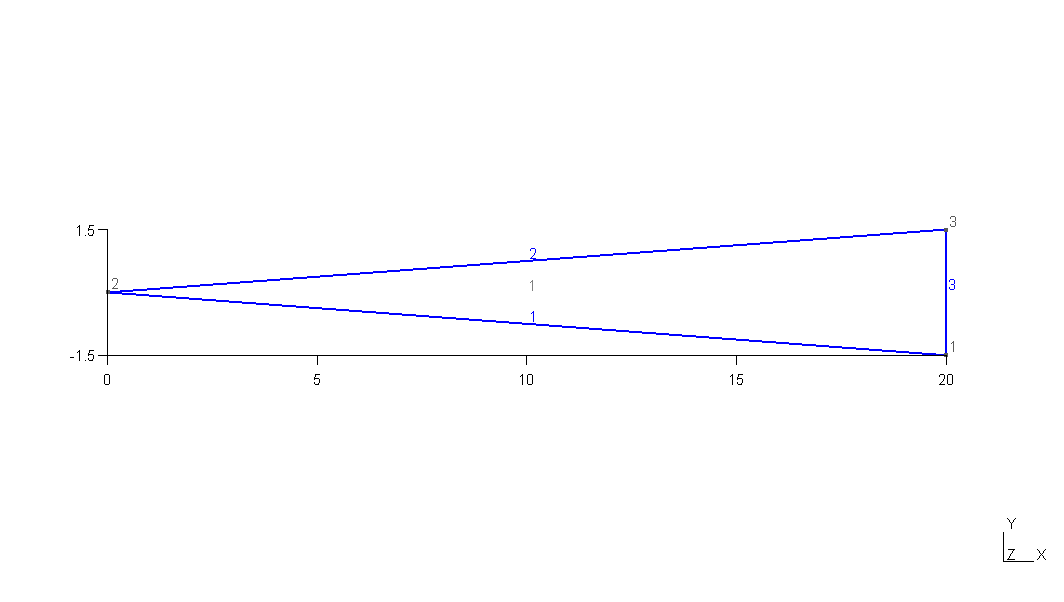
\includegraphics[width=\linewidth]{VM34/VM34_geo.png}
  \caption{Geomentry of the problem}\label{fig:awesome_image1}
\endminipage\vfill
\minipage{0.8\textwidth}
  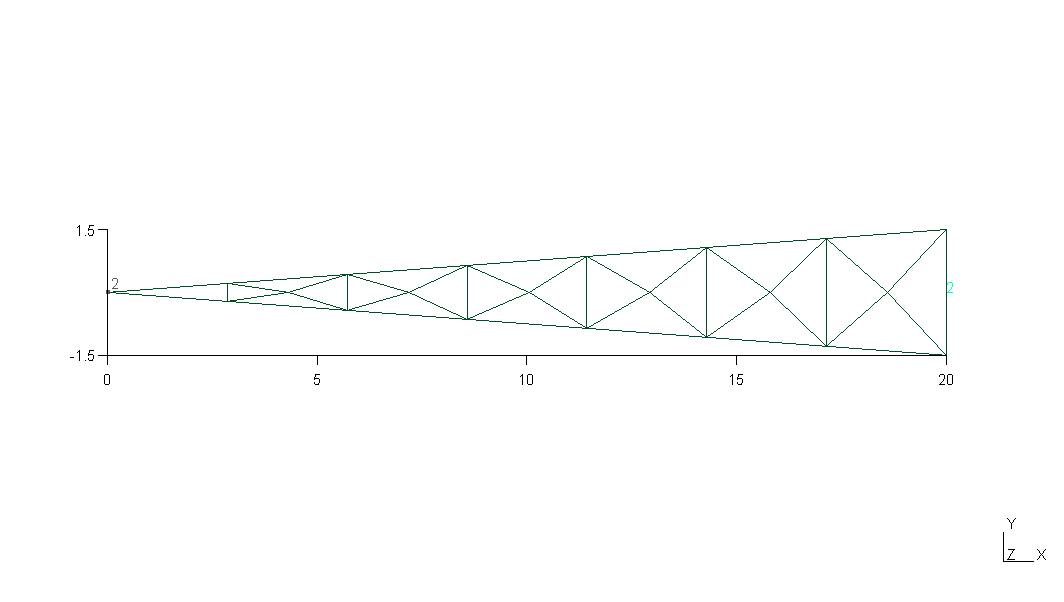
\includegraphics[width=\linewidth]{VM34/VM34_msh.png}
  \caption{Discritization}\label{fig:awesome_image2}
\endminipage\vfill
\end{figure}





\begin{table}[h!]
\renewcommand{\arraystretch}{1.5}
\centering
\caption{FEM and Boundary condition data}
\label{my-label}
\begin{tabular}{|p{25mm}l|p{20mm}|lll|p{16mm}|lll|}
\hline
\multicolumn{2}{|l|}{\cellcolor[HTML]{C0C0C0}Mesh Data} & \multicolumn{4}{l|}{\cellcolor[HTML]{C0C0C0}Direchlet Boundary} & \multicolumn{4}{l|}{\cellcolor[HTML]{C0C0C0}Neumann Boundary} \\ \hline \hline
 element size $\approx$      & 0.02 $m$                & Geo - \newline Entity      & $w$          & $\theta _ x$     & $\theta _ y $    & Geo - \newline Entity         & $F_z$        & $M_x$        & $M_y$        \\ \cline {3-10}    
Mesh file Name                   & some.msh        & line \{1,2,3,4\}                   & Fixed      & Free         & Free        & Point \{4\}                    & 10 $N$        &           &           \\ \hline
\end{tabular}
\end{table}
\subsubsection*{Analytically solution : }
The target analytically solution given is 0.042677 $In$ at load applied location. 
\newpage
\subsubsection*{Result and error analysis : }

\begin{figure}[h!]
\centering
\minipage{0.8\textwidth}%
  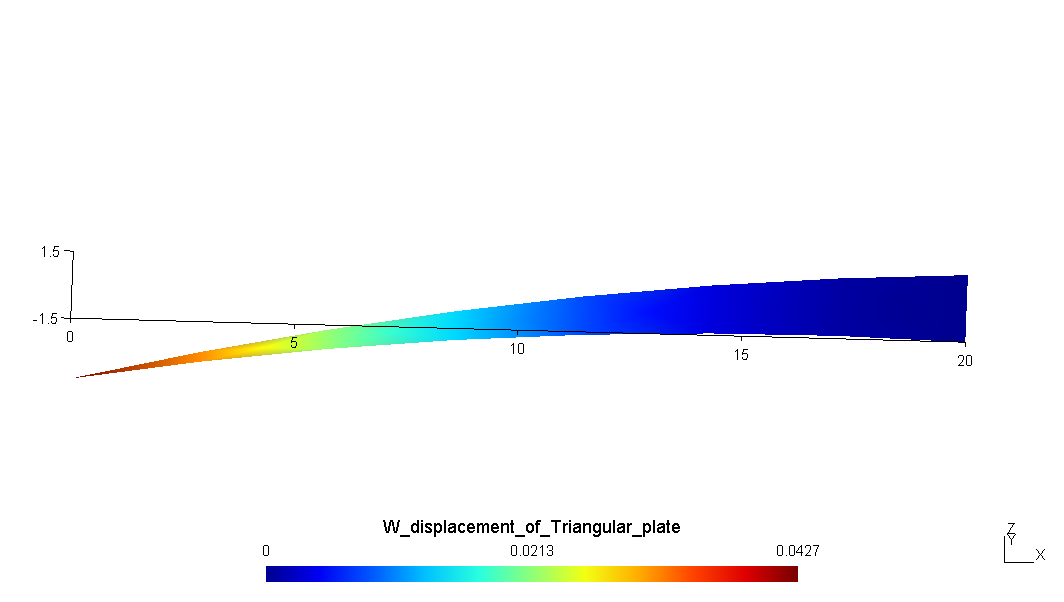
\includegraphics[width=\linewidth]{VM34/VM34_pos.png}
  \caption{FEM solution plot}\label{fig:awesome_image3}
\endminipage
\end{figure}
The maximum displacement of the domain is our solution . w displacement at point 2 is $ 0.0426677 in $.
\begin{equation}
error \% = \mid \frac{w_{analytical}-w_{FEM}}{w_{analytical}} \mid \times 100
\end{equation}

So the Error percentage is $ 0.00234 \% $. 

\end{document}